%% This document uses the class autthesis. 
%%  Refer to autthesisDocumentation.pdf for instructions on how to use the template.
%%
%% Copyright 2020, Alan T Litchfield


%% The output type is variable too
%% thesis == thesis <- this is the default, so if the type is not defined, then this is what you get
%% dissertation ==  dissertation
%% exegesis == exegesis
%% techreport == technical report
%%
%% Line spacing options are:
%%       singlespace
%%       doublespace
%%       onehalfspacing
%%
%% For programme codes, refer to autthesisDocumentation-v1.pdf

\documentclass[12pt,AK3688,techreport,doublespace]{autthesis}               %Change the options to suit the thesis

%% The packages most commonly used are defined in the class file. You can add packages below.

\usepackage{apacite}   % References are in APA format, required for AUT.
				    % For any other reference style, for example, ieee, comment out this line


% Macros for special characters that are used frequently, and to improve readability in the code
% Add macros as required to ease writing. This is a sample of how to set simple macros
\newcommand{\NZ}{New\nobreakspace{}Zealand}          %Inserts no-breakspace into proper noun
\newcommand{\nz}{New\nobreakspace{}Zealand}          %
\newcommand{\NZer}{New\nobreakspace{}Zealander}      %
\newcommand{\maori}{M\={a}ori}                       % adds macrons
\newcommand{\IT}{\textsc{it}}
\newcommand{\soa}{\textsc{soa}}


% Examples of how to define hyphenation rules
\hyphenation{Ko-tahi-tanga}
\hyphenation{Her-kunft}
\hyphenation{ma-ta-nga}
\hyphenation{Ur-sp-rung}
\hyphenation{Zim-mer-man}

% Specify the graphics path
\graphicspath{{images/}}


%% You will need to provide drafts of your chapters to your supervisor as you progress.
%% The option below allows you to print out one chapter, without all the other chapters and front/end
%% matter. Just change the file name in the braces below and uncomment the line.
%% Before running this, you need to have generated the whole thesis first.

%\ChapterProof{includes/LitReview}

\begin{document}
\author{Fred Spoons}
\title{The thesis title}
\submitdate{Change the Submission Date to suit your needs}  %% This is a manual entry because your submission date may vary from when you last generate your pdf
\dept{School of Engineering, Computer and Mathematical Sciences}
\faculty{Faculty of Design and Creative Technologies}
\primarysupervisor{Prof. P Supervisor}
%\secondarysupervisor{Prof. S Supervisor}
%\thirdsupervisor{Prof. T Supervisor}  %optional third supervisor

\abstracttext{%
\emph{Delete and replace this text}

This thesis answers all those questions others thought would be too hard. }

\acknowtext{%
\emph{Delete and replace this text. }

Where appropriate, a brief acknowledgement of any substantial assistance received should be included on a separate page inserted in sequence. The acknowledgement should list the names of all those persons who have provided substantial assistance with the research and the nature of that assistance which may relate, for example to the:
\begin{itemize*}
\item Supervisory team;
\item  Sponsorship of the research;
\item  Collection of data;
\item Processing of the data including the selection and use of particular statistical
techniques;
\item  Interpretation of the results of the statistical analysis;
\item Editing of the thesis/dissertation;
\item Use of graphics in the thesis/dissertation;
\item Word processing of the thesis/dissertation.
\end{itemize*}

If the thesis/dissertation/exegesis reports on research involving humans or human biological materials or involving animals, acknowledgement of ethics approval by the relevant ethics committee(s) should be stated in the acknowledgements section, including the ethics application number and date of approval.}

\deditext{%
\emph{Delete and replace this text.}

To remove this page, change \texttt{dedipagetrue} to \texttt{dedipagefalse}

I dedicate this study to...}

\iptext{%
\emph{Delete and replace this text}

To remove this page, change \texttt{ippagetrue} to \texttt{ippagefalse}

If there is material in the thesis/dissertation/exegesis which could or does have implications for the intellectual property rights of the student, the University, a sponsor of the research or some other person or body, those implications should be stated on this page.}

\conftext{%
\emph{Delete and replace this text}

To remove this page, change \texttt{confpagetrue} to \texttt{confpagefalse}

If there is material in the thesis/dissertation which is confidential for commercial or other reasons, either for a specified period or indefinitely, the period of its confidentiality and the reasons for its confidentiality should be specified under the heading “Confidential Material” on a separate page inserted in sequence.
Confidential material will normally be provided in a separate annex to the thesis/ dissertation/exegesis.
The Application for Embargo Form (PGR16) must be bound into all copies being lodged for examination and all final bound copies.}


%% This page is for listing publications you have produced during the research. If you have  none
%% then change \pubspagetrue{} to \pubspagefalse{} below
\pubstext{%
\emph{Delete and replace the text in this list}

To remove this page, change \texttt{pubspagetrue} to \texttt{pubspagefalse}

\begin{outdent}
\item Laudon, K. \&{} Laudon, J. (2006) Management Information Systems: Managing the Digital Firm, 9th ed. Prentice Hall
\item Walker, J. (1996) Typical UNIVAC 1108 Prices: 1968 Retrieved from \url{http://www.fourmilab.ch/documents/univac/config1108.html}
\end{outdent}}

%% Change the values below from true/false to false/true to enable/disable these 
%% optional pages
\abstractpagetrue{}
\acknowpagetrue{}
\dedipagefalse{}
\declpagetrue{}
\figurespagetrue{}
\tablespagetrue{}
\pubspagetrue{}
\ippagetrue{}
\confpagetrue{}

%% Front matter commands 
\beforeabstract{}
\afterabstract{}
\afterpreface{}


%% Putting the included chapters into a separate folder greatly eases the overall organisation

\AUTChapter{Introduction} \label{chap:intro}
\section{Introduction}
\nobreak
This is the introduction chapter. \marginNote{This is an example of a margin note, say to highlight something for your supervisor to look at} Note that the chapter titles are noted as \texttt{myChapter}. Read the class file to see how sample chapters can be printed. For the marginal note, use the command 
\begin{verbatim}
\marginNote{...}
\end{verbatim}

%\begin{comment}
This is an example of a cross reference to a figure, Fig.~\ref{fig:intro:graphSample} on page \pageref{fig:intro:graphSample}, however using the package varioref, we get Fig.~		\vref{fig:intro:graphSample}.
%\end{comment}

\begin{figure}[ht] %  figure placement: here, top, bottom, or page
   \centering
   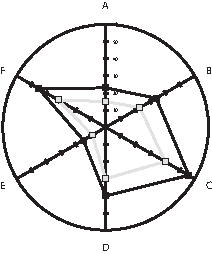
\includegraphics[width=0.3\linewidth]{graphSample} 
   \caption[Sample image]{This is a sample image file}
   \label{fig:intro:graphSample}
\end{figure}

\newpage{}
\section{Table styles}

\begin{table}[ht]
	\caption[Principle-Based Method of Systems Analysis]{Principle-Based Method of Systems Analysis Method \emph{\protect\cite{Alter2002}}} \label{tab:pbmsa}
	\centering\RaggedRight
	\begin{tabular}[t]{p{4cm}p{9cm}}
	\toprule
	\textbf{Systems analysis step} & \textbf{Steps in \textsc{pbmsa}} \\
	\hline
	1. Define the problem & Define the problem and Work System together \\
	\hline
	\parbox[t]{\linewidth}{2. Design potential improvements} & \parbox[t]{\linewidth}{Use each Work Principle in turn as a lens for summarising the current situation and search for possible improvements. 
	\begin{description} 
	\item[Principle 1] Please the Customers
	\item[Principle 2] Perform the work efficiently
	\item[Principle 3] Serve the Participants
	\item[Principle 4] Create value from information
	\item[Principle 5] Minimise effort absorbed by technology
	\item[Principle 6] Take full advantage of infrastructure
	\item[Principle 7] Minimise unintended conflicts and risks
	\item[Principle 8] Support organisational strategy
	\item[Principle 9] Maintain balance between Work System elements
	\end{description}}\\ 
	\hline
	3. Decide what to do & Make a recommendation that addresses the problem while supporting the organisation's priorities. \\
	\bottomrule
	\end{tabular}
\end{table}

This is a link to Fig.~\vref{fig:intro:graphSample}.

\singlespacing
\begin{longtable}[t]{c p{6cm} l}
\caption[Extended version of Work System Principles]{Extended version of Work System Principles \\ \indent{}\emph{Source: \protect\cite<Adapted from>[Table 2, pp.~1607--8]{Alter2004}} \label{tab:ExtendedWSPrinciples}}\\
\toprule
& \textbf{Work system principle} & \textbf{Related Work System element}\\
\hline
\endfirsthead

\caption[]{Extended version\dots{} \emph{(continued)}}\\
\toprule
& \textbf{Work system principle} & \textbf{Related Work System element}\\
\hline
\endhead

\hline
& & \hfill\emph{Continued over page} \\
\bottomrule
\endfoot

\bottomrule
\endlastfoot

& \textbf{1:} Please the customers. & Customers and products \& services \\
\dag{}\footnote{Those principles that have been added in Alter's revision are indicated with a \dag{} symbol.} & \textbf{2:} Balance priorities of different customers. & Customers and products \\
\dag{} & \textbf{3:} Match process flexibility with product variability. & Product and work practices\footnote{Previously referred to as Business Processes, Alter has changed term to ``work practices.''} \\
& \textbf{4:} Perform the work efficiently. & Work practices \\
\dag{} & \textbf{5:} Encourage appropriate use of judgement. & Work practices \\
\dag{} & \textbf{6:} Control variances (problems) at their source. & Work practices \\
\dag{} & \textbf{7:} Monitor the quality of both inputs and outputs. & Work practices \\
\dag{} & \textbf{8:} Boundaries between business process steps should facilitate control & Work practices \\
\dag{} & \textbf{9:} Match the work practices with the participants. & Work practices and participants \\
& \textbf{10:} Serve the participants & Participants \\
\dag{} & \textbf{11:} Align participant incentives with system goals & Participants \\
\dag{} & \textbf{12:} Provide information where it will affect action & Information and work practices \\
\dag{} & \textbf{13:} Protect information from inappropriate use & Information \\
\dag{} & \textbf{14:} Use appropriate technology & Technology and work practices \\
& \textbf{15:} Minimise effort consumed by technology & Technology \\
& \textbf{16:} Take full advantage of infrastructure & Infrastructure \\
& \textbf{17:} Minimise unnecessary conflict with the external environment & Environment\footnote{Previously referred to as Context, Environment is distinct from Infrastructure and Technology whereas Context could be confused with both.} \\
& \textbf{18:} Support the firm's strategy & Strategy \\
& \textbf{19:} Minimise unnecessary risks & System as a whole \\
& \textbf{20:} Maintain balance between work system elements & System as a whole \\
\dag{} & \textbf{21:} Maintain the ability to adapt, change, and grow. & System as a whole \\
\end{longtable}
\doublespacing

A sample citation: \cite{Bannon1997}.

apacite specific examples:
\begin{itemize} 
\item \citeA{Bannon1997}
\item \citeNP{Bannon1997}
\end{itemize}

\newpage{}
\section{Listing styles}
\subsection{Itemised list}
This listing style uses \texttt{itemize*} to pull the increased line spacing closer.
\begin{itemize*}
\item Lorem ipsum dolor sit amet, consetetur sadipscing elitr, sed diam nonumy eirmod tempor invidunt ut labore et dolore magna aliquyam erat, sed diam voluptua. '
\item At vero eos et accusam et justo duo dolores et ea rebum. 
\item Stet clita kasd gubergren, no sea takimata sanctus est Lorem ipsum dolor sit amet. Lorem ipsum dolor sit amet, consetetur sadipscing elitr, sed diam nonumy eirmod tempor invidunt ut labore et dolore magna aliquyam erat, sed diam voluptua.
\end{itemize*}

\subsection{Enumerated list}
This listing style uses \texttt{enumerate*} to pull the increased line spacing closer.
\begin{enumerate*}
\item Lorem ipsum dolor sit amet, consetetur sadipscing elitr, sed diam nonumy eirmod tempor invidunt ut labore et dolore magna aliquyam erat, sed diam voluptua. '
	\begin{enumerate*}
	\item Lorem ipsum dolor sit amet, consetetur sadipscing elitr, sed diam nonumy eirmod tempor invidunt ut labore et dolore magna aliquyam erat, sed diam voluptua. '
	\item At vero eos et accusam et justo duo dolores et ea rebum. 
	\item Stet clita kasd gubergren, no sea takimata sanctus est Lorem ipsum dolor sit amet. Lorem ipsum dolor sit amet, consetetur sadipscing elitr, sed diam nonumy eirmod tempor invidunt ut labore et dolore magna aliquyam erat, sed diam voluptua.
	\end{enumerate*}
\item At vero eos et accusam et justo duo dolores et ea rebum. 
\item Stet clita kasd gubergren, no sea takimata sanctus est Lorem ipsum dolor sit amet. Lorem ipsum dolor sit amet, consetetur sadipscing elitr, sed diam nonumy eirmod tempor invidunt ut labore et dolore magna aliquyam erat, sed diam voluptua.
\end{enumerate*}

\subsection{Description list}
This listing style uses \texttt{description*} to pull the increased line spacing closer.
\begin{description*}
\item[Lorem ipsum] dolor sit amet, consetetur sadipscing elitr, sed diam nonumy eirmod tempor invidunt ut labore et dolore magna aliquyam erat, sed diam voluptua. '
	\begin{enumerate*}
	\item Lorem ipsum dolor sit amet, consetetur sadipscing elitr, sed diam nonumy eirmod tempor invidunt ut labore et dolore magna aliquyam erat, sed diam voluptua. '
	\item At vero eos et accusam et justo duo dolores et ea rebum. 
	\item Stet clita kasd gubergren, no sea takimata sanctus est Lorem ipsum dolor sit amet. Lorem ipsum dolor sit amet, consetetur sadipscing elitr, sed diam nonumy eirmod tempor invidunt ut labore et dolore magna aliquyam erat, sed diam voluptua.
	\end{enumerate*}
\item[At vero eos et accusam] et justo duo dolores et ea rebum. 
\item[Stet clita kasd gubergren] no sea takimata sanctus est Lorem ipsum dolor sit amet. Lorem ipsum dolor sit amet, consetetur sadipscing elitr, sed diam nonumy eirmod tempor invidunt ut labore et dolore magna aliquyam erat, sed diam voluptua.
\end{description*}

\section{Some various citation styles}
\nobreak
Lorem ipsum dolor sit amet, consetetur sadipscing elitr, sed diam nonumy eirmod tempor invidunt ut labore et dolore magna aliquyam erat, sed diam voluptua \cite{Quine2004}. At vero eos et accusam et justo duo dolores et ea rebum. Stet clita kasd gubergren, no sea takimata sanctus est Lorem ipsum dolor sit amet \cite{Peirce1992a}. Lorem ipsum dolor sit amet, consetetur sadipscing elitr, sed diam nonumy eirmod tempor invidunt ut labore et dolore magna aliquyam erat, sed diam voluptua.

 duis autem vel eum iriure dolor in hendrerit in vulputate velit esse molestie consequat, ``vel illum dolore eu feugiat nulla facilisis at vero eros et accumsan et iusto odio dignissim qui blandit praesent luptatum zzril delenit augue duis dolore te feugait nulla facilisi'.

\section{Some verbatim code}

\begin{verbatim}
this is some code
    this code is indented
        and further indented
\end{verbatim}
\section{Conclusion}
\nobreak
Lorem ipsum dolor sit amet, consetetur sadipscing elitr, sed diam nonumy eirmod tempor invidunt ut labore et dolore magna aliquyam erat, sed diam voluptua. At vero eos et accusam et justo duo dolores et ea rebum. Stet clita kasd gubergren, no sea takimata sanctus est Lorem ipsum dolor sit amet. Lorem ipsum dolor sit amet, consetetur sadipscing elitr, sed diam nonumy eirmod tempor invidunt ut labore et dolore magna aliquyam erat, sed diam voluptua.

Duis autem vel eum iriure dolor in hendrerit in vulputate velit esse molestie consequat, vel illum dolore eu feugiat nulla facilisis at vero eros et accumsan et iusto odio dignissim qui blandit praesent luptatum zzril delenit augue duis dolore te feugait nulla facilisi.

Lorem ipsum dolor sit amet, consetetur sadipscing elitr, sed diam nonumy eirmod tempor invidunt ut labore et dolore magna aliquyam erat, sed diam voluptua. At vero eos et accusam et justo duo dolores et ea rebum. Stet clita kasd gubergren, no sea takimata sanctus est Lorem ipsum dolor sit amet. Lorem ipsum dolor sit amet, consetetur sadipscing elitr, sed diam nonumy eirmod tempor invidunt ut labore et dolore magna aliquyam erat, sed diam voluptua.

Duis autem vel eum iriure dolor in hendrerit in vulputate velit esse molestie consequat, vel illum dolore eu feugiat nulla facilisis at vero eros et accumsan et iusto odio dignissim qui blandit praesent luptatum zzril delenit augue duis dolore te feugait nulla facilisi.

Lorem ipsum dolor sit amet, consetetur sadipscing elitr, sed diam nonumy eirmod tempor invidunt ut labore et dolore magna aliquyam erat, sed diam voluptua. At vero eos et accusam et justo duo dolores et ea rebum. Stet clita kasd gubergren, no sea takimata sanctus est Lorem ipsum dolor sit amet. Lorem ipsum dolor sit amet, consetetur sadipscing elitr, sed diam nonumy eirmod tempor invidunt ut labore et dolore magna aliquyam erat, sed diam voluptua.

Duis autem vel eum iriure dolor in hendrerit in vulputate velit esse molestie consequat, vel illum dolore eu feugiat nulla facilisis at vero eros et accumsan et iusto odio dignissim qui blandit praesent luptatum zzril delenit augue duis dolore te feugait nulla facilisi.

\AUTChapter{Literature Review} \label{chap:litrev}

\section{Introduction}\label{sec:Introduction}

The literature review design of this PHD research constitutes of 3 parts, 2 systematic literature reviews (SLR) on the topics ‘Big data reference architectures’ and ‘E-commerce systems” and one generic literature review on the topic ‘Big data’.

Systematic literature reviews take shape by embarking on an extensive search for topic-related articles within the years 2010-2020. Most literature chosen for the purposes of this research are within the years 2016-2020 as they provided with recent, and more relevant information. Albeit, some old studies dating back to 2010, helped clarifying some basic matters that existed and how they correlated to big data. world most renowned online libraries for quality research have been selected such as IEEE, MIS Quarterly, Science Direct, Elsevier, Springer, ACM, AISeL and Emerald insight.

Every library provided with a vast sea of research and inordinate amount of information to absorb. Arguably, different publications provided with different sort of mental framework and so did the authors. For instance, it’s been found that many high-quality information system researches are published in MIS quarterly, whereas Elsevir and SpringerLink provided with quality big-data literature.

A combination of long-tail and short-tail keywords are chosen to target literature that are related to the current state of art. Keywords chosen for ‘Big data reference architectures’ SLR are ‘big data reference architectures’, and ‘reference architectures. Keywords chosen for ‘E-commerce systems’ are ‘e-commerce system architectures’, ‘smart e-commerce systems’, and ‘e-commerce and big data’. Each systematic literature review is conducted in a span of three weeks.

In what follows, first the generic big data literature review will be conducted, second ‘big data reference architecture’ SLR and finally ‘E-commerce systems’ SLR will take place.

\section{State of the art}\label{sec:State of the art}

We’ve come a long way with technology, and specifically software development. In fact, the rapid advancements left many spaced out. From the emergence of the first computer Eniac in 1946 to 8-core 5.0GHz processing core speed in 2019; From document-oriented waterfalls to agile two-weeks sprints; from punch cards to fancy transpilers  and dynamic programming languages.  Computers were first perceived as calculation engines and has been used to focus entirely on algorithms and mathematics. It was during the mid-1950, that it became commercially available and businessmen start to pick it up to produce value for business. Along the lines, once people started using computers for real-life purposes, many leftover data has been produced, as these data increased, people started realizing the value of it and began to store it \cite{Grad2009}.

That’s where the industry came up with a concept of a Database Management System (DBMS), and humanity began to store data for various purposes. In 1968, as a result of a NATO-sponsored conference, the term software engineering emerged, referring to a highly systematic approach to software development and maintenance \cite{Wirth2008}.

Since the beginning of 1968, the advancement began on the areas of tools generation, testing, automation and systematizing. During the same years, in 1960s the history of computer hardware started by conversion of vacuum tubes to solid-states. Todays, the word ‘bug’ is quite a common phrase among engineers and programmers to refer to a fault, failure or a flaw. We ow this word to a literal moth that were caught inside a tube before the transition to solid states. It is hardly conceivable that we’ve progressed from absolutely no understanding for data to devices that can produce zettabytes of them in a span of 60 years. Along this track, software engineering has passed several major phases. Recent polyglot approaches with nascent lambda functions, functional paradigms and micro-services have come to take the industry by storm. This is the only time in human history, where the computing resources and the necessary data is available to harness the hidden patterns behind every momentum or dynamism. Being so focused on development of more maintainable and scalable software, and microchips and hardware’s and devices that can perform faster and last longer, we have lost the track of the output of all these entities and peripherals, and that’s the void that current industry is facing. Abundance of computer power, the emergence of open source community, and the ubiquity of internet has brought us with a new material to harness. A material, that is complex and random in nature.

It was not until 2005 that the term big data has been coined \cite{Long2015}, and Web 2.0 emerged which referred to a large set of data that is impossible to process with the traditional data management systems. Within the same year, Yahoo created Hadoop, Google came up with MapReduce. In 2009, the Indian government took a revolutionary step and decided to take an iris scan of its 1.2 billion inhabitants. In 2011 McKinesy published the title “Big Data: the next frontier of innovation” and startups and companies started investing heavily in this field. The big data revolution is ahead of us, and yet there is a big chasm both in practice and academia \cite{mckinsey2011big}.

\footnote{A transpiler is a sort of a compiler that translates source codes from one language to another, or another version of the same language. For example Babel (a Javascript Library ) transpiles the latest syntax of Javascript ( ES6 ) into older version of it ( ES5 ), thus all the browsers can support the system.}

\section{Big data}\label{Big Data}
\subsection{What is big data?}\label{What is big data?}

To define big data for the course of this PHD thesis, we will first look at available definitions in academia.

\citeauthor{Kaisler2013} define big data as “the amount of data which is beyond technology’s capability to store, manage and process efficiently.\citeauthor{Srivastava2018} referred to big data as “the use of large data sets to handle the collection or reporting of data that serves business or other recipients in decision making”.

\citeauthor{Sagiroglu2013} define big data as “a term for massive data sets having large, more varied and complex structure with the difficulties of storing, analyzing and visualizing for further processes or results”.  Inspired by these definitions, we define big data as “an endeavor to harness the patterns behind vast amount of data for the purposes of improvement, control, and prediction of business matters”.

\section{The Hype of Emerging Technologies}

The term big data, was initially coined to refer to the gradual growth and availability of data \cite{lycett2013datafication}.

The ubiquity of digital devices and capability of users to produce different forms of data, have consolidated the interconnected links among suppliers, customers, affiliates, partners, and stakeholders \cite{Bughin2016}. With recent emergence of 5G technology and its launch in the UK, we are experiencing a fundamental network shift that is unprecedented in human history \cite{ahmad20205g}

Opposed to general belief of 5G being only faster than its elder brother 4G, 5G has come to offer bi-directional large bandwidth shaping, large broadcasting of data in gigabits which supports wearable devices with AI capabilities, pervasive networks providing ubiquitous computing (the user can be seamlessly connected to several wireless access technologies), traffic statistics, IPV6 utilization and finally 25Mbps of connectivity speed \cite{Gohil2013}.

In a world where we have the average processing power of 1.5 GHz on smart phones and up to 8 GHz on desktops running on network infrastructures that will support up to 25Mbps of transmission per second, data becomes the new oil, the atom, the dot that lays the foundation of the nexus \cite{Rad2017}. It is astonishing to witness data being produced by netizens in every second .According to live internet statistics website , there are 4 billion internet users currently active, that produce 8,522 Tweets, 920 Instagram photos, 1,540 Tumbler posts, 3,868 Skype calls, 74,993 Google searches, 79,099 Youtube videos, 2,806,143 emails, and 73,693 GB of internet traffic per second \cite{Stats2017}. That implies, if it has taken 3 seconds to read the preceding paragraph, in the interim, 221,79 GB of traffic has been produced. Howbeit, how useful are these data? And how far have we gone with harnessing its power?


\section{The Value of Big Data}

The value of big data is no longer under the hood. In fact, the concept has been repeatedly discussed in various reports, statistics, researches and conferences \cite{Chen2012}. The outburst is driven by the colossal investment of companies such as Google, Facebook, Netflix and Amazon \cite{Rada2017}.

A study of Netflix Prize recommender system provided details on employment of big data in order to induce better, more accurate results \cite{Amatriain2013}. The research has explicitly stated the notion of using various pools of data to further optimize recommendations. Data produced by queries, ratings, queues, search terms, and metadata alongside impression, social, external, demographic, location, language, and finally temporal data has been taken in use for predictive models \cite{Amatriain2013}. Using big data enforced recommendation systems, the company has managed to increase TV series consumption by the factor of four \cite{Amatriain2013}.

The Taiwanese government leveraged its national health insurance database and merged it with custom and immigration datasets to forge a big data initiative \cite{wang2020response}. This initiative resulted in improved case identification by generating real-time alerts during clinical visits. These alerts have been created by the analysis of clinical symptoms, travel history, and other data that could be found. Proactively seeking out patients that may be infected by COVID-19 was one of the reasons that Taiwanese government managed to handle the epidemic effectively.

Shell uses big data to reduce costs energy resources exploration \cite{Marr2016}. The company uploads data to analytics system and compare it with data from drilling sites around the world. The closer the results match where abundant resources have been found, the better decision will be made. Before big data, company had huge problems to identify energy resources. Waves of energies traveled through the earth’s crust registered differently on sensors, depending on whether they are travelling through gaseous material, liquids, or solid rocks. Formerly, company employed the traditional hit and miss approach to confirm the findings of the initial survey which was expensive and time-consuming.

Along the lines, Rolls Royce harness the power of big data by capturing internal data from sensors fitter on the company’s aircraft products. The data is received through a wireless transmission medium and contains multitudes of performance reports. These reports shed lights on various key phases such as take-off, engine power climax, steady state (climb and cruise), dynamisms, and maintenance \cite{Marr2016}. The company uses the data to detect degradation, to induce diagnosis and prognosis, and to minimize the false-positive as well.

\section{Datocracy}

The availability of data at an unprecedented frequency and the hidden patterns behind this nexus of interconnections has resulted in a new world, a datocratic world. Before getting further, is it essential to grasp the meaning of the new term ‘Datocracy’ proposed to correctly address the lingual needs for this research. To clarify the meaning of the word, it is helpful to understand the etymology behind the common term “Democracy”. Deomcracy comes from the combination of two ancient Greek words namely “demos” meaning ‘people’, and the post fix “-Kratia” meaning ‘to rule’. By the same line the combination of the Greek word “Datum” and the post fix “-Kratia” generates the word Datocracy, meaning “data to rule”.


\begin{figure}[h!]
    \centering
    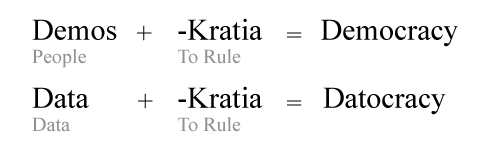
\includegraphics[width=8cm]{Datocracy.png}
    \caption{Datocracy}
    \label{fig:datocracy}
\end{figure}


\section{Ubiquity}

Recent technology shifts and the computing power that each person carries along, has brought along a new business material, a datocracy. In a conference held in Abu Dhabi in 2013, Joseph S. Nye, a former US assistance secretary of defense and a university professor at Harvard, proposed the idea of future governance in the age of information \cite{Nye2013}.

He proposed the scenario in which the central government will use big data to fortify control. On the other hand, there is an estimation of 7121 publications on the fields big data regarding different dimensions, such as mathematical techniques, decision-making techniques, data characteristics, technical challenges and adoption failures \cite{Wang2016}.

Paying clear attention to recent social, commercial and industrial trends will yield the evidence of big data ubiquity. In the domain of social network, there has been study for understanding temporal patterns of happiness by using a data set of 46 billion words contained in nearly 4.6 billion expression by 63 million unique users posted over a 33 months span \cite{Dodds2011}.

Furthermore, in another research, big data analytics and semantic network analysis were utilized to examine the largest data set collected on Twitter during 2012 U.S presidential election \cite{Guo2015}. The study concluded that the news media could determine the public’s identification of a certain candidate.

Other academicians have used big data to develop a novel distributed community structure mining framework. The framework makes use of local information data alongside MapReduce, and well-known algorithms such as FastGN, and Radetal to address scalability, velocity, and accuracy \cite{Jin2015}. On a bigger, more social-oriented studies, there has been researches regarding the overall well-being Turkish citizens by adopting a sentiment analysis model \cite{Durahim2015}.

Along the lines, the very sentiment analysis model has been taken by other researchers to discover general knowledge from social media \cite{Bohlouli2015}, and to evaluate and infer enhanced marketing advantage and to shed lights on areas in which the business is leading and lagging to further improve customer-business relation \cite{He2015}.

Similar researches have been conducted by analyzing suspended spam accounts on Twitter in terms of the profile’s properties and interactions. These researchers were aimed to point out spammers and malicious users by using big data \cite{Almaatouq2016}. \citeauthor{Chainey2008} have conducted a research on hotspot mapping and its usage to identify spatial patterns of crime. The study concluded that by utilizing a data from the past, hotspot mappings can identify where crimes most densely occur. From there on, there has been the proposition of target enforcement and prevention resources in the crime areas for mitigating crimes.

By the same token, \cite{Li2012} used a large dataset from the bank of Taiwan and developed a big data system to identify signs and patterns of fraudulent accounts. They’ve developed a detection system by applying the Bayesian Classification and Association Rule. Along the lines, there has been other researches to predict negative behaviors spreading dynamics \cite{Liao2015}, emotional response detection by browsing Facebook \cite{Lin2015}, as well as identifying the impacts of national security by using the US intelligent community datasets \cite{Crampton2015}.

A wander into different areas provides with interesting ideas about how far the progress has been with the adoption of big data and proves a truly datocratic world. One good example is a comparative study conducted to document how big data can help with multifaceted aspects of international accreditations for two universities, namely Plekhanov Russian University of Economic and HAN University of Applied Science (Arnhem Business School) \cite{Popescu2019}.

In addition, \cite{Zhang2019a} conducted a research on the application of big data for tours and creative agencies. The objective of the study was to extract behavioral data and to form strategic objects that can be later applied for business benefit.

As witnessed hereinabove, there are abundant number of researches on the application of big data in various industries. Table 1 portrays an overview of the aforementioned studies and even further.

\begin{center}
    \begin{tabular}{|c|c|c|}
        \hline
        Contibution & \multicolumn{2}{c|}{Multi-column}                                              \\

        \hline
        Contibution & Research Focus                    & \multirow{2}{*}{\begin{turn}{-90} Test 90 \end{turn}} \\

        Contibution & Research Focus                    &                                            \\

        Contibution & Research Focus                    &                                            \\

        \hline
    \end{tabular}
\end{center}




\AUTChapter{Method} \label{chap:method}
\nobreak
\section{Introduction}
\nobreak
Lorem ipsum dolor sit amet, consetetur sadipscing elitr, sed diam nonumy eirmod tempor invidunt ut labore et dolore magna aliquyam erat, sed diam voluptua. At vero eos et accusam et justo duo dolores et ea rebum. Stet clita kasd gubergren, no sea takimata sanctus est Lorem ipsum dolor sit amet. Lorem ipsum dolor sit amet, consetetur sadipscing elitr, sed diam nonumy eirmod tempor invidunt ut labore et dolore magna aliquyam erat, sed diam voluptua.

Duis autem vel eum iriure dolor in hendrerit in vulputate velit esse molestie consequat, vel illum dolore eu feugiat nulla facilisis at vero eros et accumsan et iusto odio dignissim qui blandit praesent luptatum zzril delenit augue duis dolore te feugait nulla facilisi.

Lorem ipsum dolor sit amet, consetetur sadipscing elitr, sed diam nonumy eirmod tempor invidunt ut labore et dolore magna aliquyam erat, sed diam voluptua. At vero eos et accusam et justo duo dolores et ea rebum. Stet clita kasd gubergren, no sea takimata sanctus est Lorem ipsum dolor sit amet. Lorem ipsum dolor sit amet, consetetur sadipscing elitr, sed diam nonumy eirmod tempor invidunt ut labore et dolore magna aliquyam erat, sed diam voluptua.

Duis autem vel eum iriure dolor in hendrerit in vulputate velit esse molestie consequat, vel illum dolore eu feugiat nulla facilisis at vero eros et accumsan et iusto odio dignissim qui blandit praesent luptatum zzril delenit augue duis dolore te feugait nulla facilisi.

Lorem ipsum dolor sit amet, consetetur sadipscing elitr, sed diam nonumy eirmod tempor invidunt ut labore et dolore magna aliquyam erat, sed diam voluptua. At vero eos et accusam et justo duo dolores et ea rebum. Stet clita kasd gubergren, no sea takimata sanctus est Lorem ipsum dolor sit amet. Lorem ipsum dolor sit amet, consetetur sadipscing elitr, sed diam nonumy eirmod tempor invidunt ut labore et dolore magna aliquyam erat, sed diam voluptua.

Duis autem vel eum iriure dolor in hendrerit in vulputate velit esse molestie consequat, vel illum dolore eu feugiat nulla facilisis at vero eros et accumsan et iusto odio dignissim qui blandit praesent luptatum zzril delenit augue duis dolore te feugait nulla facilisi.
Lorem ipsum dolor sit amet, consetetur sadipscing elitr, sed diam nonumy eirmod tempor invidunt ut labore et dolore magna aliquyam erat, sed diam voluptua. At vero eos et accusam et justo duo dolores et ea rebum. Stet clita kasd gubergren, no sea takimata sanctus est Lorem ipsum dolor sit amet. Lorem ipsum dolor sit amet, consetetur sadipscing elitr, sed diam nonumy eirmod tempor invidunt ut labore et dolore magna aliquyam erat, sed diam voluptua.

Duis autem vel eum iriure dolor in hendrerit in vulputate velit esse molestie consequat, vel illum dolore eu feugiat nulla facilisis at vero eros et accumsan et iusto odio dignissim qui blandit praesent luptatum zzril delenit augue duis dolore te feugait nulla facilisi.

Lorem ipsum dolor sit amet, consetetur sadipscing elitr, sed diam nonumy eirmod tempor invidunt ut labore et dolore magna aliquyam erat, sed diam voluptua. At vero eos et accusam et justo duo dolores et ea rebum. Stet clita kasd gubergren, no sea takimata sanctus est Lorem ipsum dolor sit amet. Lorem ipsum dolor sit amet, consetetur sadipscing elitr, sed diam nonumy eirmod tempor invidunt ut labore et dolore magna aliquyam erat, sed diam voluptua.

Duis autem vel eum iriure dolor in hendrerit in vulputate velit esse molestie consequat, vel illum dolore eu feugiat nulla facilisis at vero eros et accumsan et iusto odio dignissim qui blandit praesent luptatum zzril delenit augue duis dolore te feugait nulla facilisi.

\section{Conclusion} \label{sec:Method:Conclusion}
\nobreak
Lorem ipsum dolor sit amet, consetetur sadipscing elitr, sed diam nonumy eirmod tempor invidunt ut labore et dolore magna aliquyam erat, sed diam voluptua. At vero eos et accusam et justo duo dolores et ea rebum. Stet clita kasd gubergren, no sea takimata sanctus est Lorem ipsum dolor sit amet. Lorem ipsum dolor sit amet, consetetur sadipscing elitr, sed diam nonumy eirmod tempor invidunt ut labore et dolore magna aliquyam erat, sed diam voluptua.

Duis autem vel eum iriure dolor in hendrerit in vulputate velit esse molestie consequat, vel illum dolore eu feugiat nulla facilisis at vero eros et accumsan et iusto odio dignissim qui blandit praesent luptatum zzril delenit augue duis dolore te feugait nulla facilisi.

\AUTChapter{Analysis} \label{chap:analysis}
\nobreak
\section{Introduction}
\nobreak
Lorem ipsum dolor sit amet, consetetur sadipscing elitr, sed diam nonumy eirmod tempor invidunt ut labore et dolore magna aliquyam erat, sed diam voluptua. At vero eos et accusam et justo duo dolores et ea rebum. Stet clita kasd gubergren, no sea takimata sanctus est Lorem ipsum dolor sit amet. Lorem ipsum dolor sit amet, consetetur sadipscing elitr, sed diam nonumy eirmod tempor invidunt ut labore et dolore magna aliquyam erat, sed diam voluptua.

Duis autem vel eum iriure dolor in hendrerit in vulputate velit esse molestie consequat, vel illum dolore eu feugiat nulla facilisis at vero eros et accumsan et iusto odio dignissim qui blandit praesent luptatum zzril delenit augue duis dolore te feugait nulla facilisi.

Lorem ipsum dolor sit amet, consetetur sadipscing elitr, sed diam nonumy eirmod tempor invidunt ut labore et dolore magna aliquyam erat, sed diam voluptua. At vero eos et accusam et justo duo dolores et ea rebum. Stet clita kasd gubergren, no sea takimata sanctus est Lorem ipsum dolor sit amet. Lorem ipsum dolor sit amet, consetetur sadipscing elitr, sed diam nonumy eirmod tempor invidunt ut labore et dolore magna aliquyam erat, sed diam voluptua.

Duis autem vel eum iriure dolor in hendrerit in vulputate velit esse molestie consequat, vel illum dolore eu feugiat nulla facilisis at vero eros et accumsan et iusto odio dignissim qui blandit praesent luptatum zzril delenit augue duis dolore te feugait nulla facilisi.

Lorem ipsum dolor sit amet, consetetur sadipscing elitr, sed diam nonumy eirmod tempor invidunt ut labore et dolore magna aliquyam erat, sed diam voluptua. At vero eos et accusam et justo duo dolores et ea rebum. Stet clita kasd gubergren, no sea takimata sanctus est Lorem ipsum dolor sit amet. Lorem ipsum dolor sit amet, consetetur sadipscing elitr, sed diam nonumy eirmod tempor invidunt ut labore et dolore magna aliquyam erat, sed diam voluptua.

Duis autem vel eum iriure dolor in hendrerit in vulputate velit esse molestie consequat, vel illum dolore eu feugiat nulla facilisis at vero eros et accumsan et iusto odio dignissim qui blandit praesent luptatum zzril delenit augue duis dolore te feugait nulla facilisi.

\section{Conclusion} \label{sec:analysis:conclusion}
\nobreak{}
Lorem ipsum dolor sit amet, consetetur sadipscing elitr, sed diam nonumy eirmod tempor invidunt ut labore et dolore magna aliquyam erat, sed diam voluptua. At vero eos et accusam et justo duo dolores et ea rebum. Stet clita kasd gubergren, no sea takimata sanctus est Lorem ipsum dolor sit amet. Lorem ipsum dolor sit amet, consetetur sadipscing elitr, sed diam nonumy eirmod tempor invidunt ut labore et dolore magna aliquyam erat, sed diam voluptua.

Duis autem vel eum iriure dolor in hendrerit in vulputate velit esse molestie consequat, vel illum dolore eu feugiat nulla facilisis at vero eros et accumsan et iusto odio dignissim qui blandit praesent luptatum zzril delenit augue duis dolore te feugait nulla facilisi.

\AUTChapter{Discussion} \label{chap:Discussion}
\nobreak
\section{Introduction}
\nobreak
Lorem ipsum dolor sit amet, consetetur sadipscing elitr, sed diam nonumy eirmod tempor invidunt ut labore et dolore magna aliquyam erat, sed diam voluptua. At vero eos et accusam et justo duo dolores et ea rebum. Stet clita kasd gubergren, no sea takimata sanctus est Lorem ipsum dolor sit amet. Lorem ipsum dolor sit amet, consetetur sadipscing elitr, sed diam nonumy eirmod tempor invidunt ut labore et dolore magna aliquyam erat, sed diam voluptua.

Duis autem vel eum iriure dolor in hendrerit in vulputate velit esse molestie consequat, vel illum dolore eu feugiat nulla facilisis at vero eros et accumsan et iusto odio dignissim qui blandit praesent luptatum zzril delenit augue duis dolore te feugait nulla facilisi.Lorem ipsum dolor sit amet, consetetur sadipscing elitr, sed diam nonumy eirmod tempor invidunt ut labore et dolore magna aliquyam erat, sed diam voluptua. At vero eos et accusam et justo duo dolores et ea rebum. Stet clita kasd gubergren, no sea takimata sanctus est Lorem ipsum dolor sit amet. Lorem ipsum dolor sit amet, consetetur sadipscing elitr, sed diam nonumy eirmod tempor invidunt ut labore et dolore magna aliquyam erat, sed diam voluptua.

Duis autem vel eum iriure dolor in hendrerit in vulputate velit esse molestie consequat, vel illum dolore eu feugiat nulla facilisis at vero eros et accumsan et iusto odio dignissim qui blandit praesent luptatum zzril delenit augue duis dolore te feugait nulla facilisi.Lorem ipsum dolor sit amet, consetetur sadipscing elitr, sed diam nonumy eirmod tempor invidunt ut labore et dolore magna aliquyam erat, sed diam voluptua. At vero eos et accusam et justo duo dolores et ea rebum. Stet clita kasd gubergren, no sea takimata sanctus est Lorem ipsum dolor sit amet. Lorem ipsum dolor sit amet, consetetur sadipscing elitr, sed diam nonumy eirmod tempor invidunt ut labore et dolore magna aliquyam erat, sed diam voluptua.

Duis autem vel eum iriure dolor in hendrerit in vulputate velit esse molestie consequat, vel illum dolore eu feugiat nulla facilisis at vero eros et accumsan et iusto odio dignissim qui blandit praesent luptatum zzril delenit augue duis dolore te feugait nulla facilisi.Lorem ipsum dolor sit amet, consetetur sadipscing elitr, sed diam nonumy eirmod tempor invidunt ut labore et dolore magna aliquyam erat, sed diam voluptua. At vero eos et accusam et justo duo dolores et ea rebum. Stet clita kasd gubergren, no sea takimata sanctus est Lorem ipsum dolor sit amet. Lorem ipsum dolor sit amet, consetetur sadipscing elitr, sed diam nonumy eirmod tempor invidunt ut labore et dolore magna aliquyam erat, sed diam voluptua.

Duis autem vel eum iriure dolor in hendrerit in vulputate velit esse molestie consequat, vel illum dolore eu feugiat nulla facilisis at vero eros et accumsan et iusto odio dignissim qui blandit praesent luptatum zzril delenit augue duis dolore te feugait nulla facilisi.Lorem ipsum dolor sit amet, consetetur sadipscing elitr, sed diam nonumy eirmod tempor invidunt ut labore et dolore magna aliquyam erat, sed diam voluptua. At vero eos et accusam et justo duo dolores et ea rebum. Stet clita kasd gubergren, no sea takimata sanctus est Lorem ipsum dolor sit amet. Lorem ipsum dolor sit amet, consetetur sadipscing elitr, sed diam nonumy eirmod tempor invidunt ut labore et dolore magna aliquyam erat, sed diam voluptua.

Duis autem vel eum iriure dolor in hendrerit in vulputate velit esse molestie consequat, vel illum dolore eu feugiat nulla facilisis at vero eros et accumsan et iusto odio dignissim qui blandit praesent luptatum zzril delenit augue duis dolore te feugait nulla facilisi.

\section{Conclusion} \label{sec:democrat:conclusion}
\nobreak
Lorem ipsum dolor sit amet, consetetur sadipscing elitr, sed diam nonumy eirmod tempor invidunt ut labore et dolore magna aliquyam erat, sed diam voluptua. At vero eos et accusam et justo duo dolores et ea rebum. Stet clita kasd gubergren, no sea takimata sanctus est Lorem ipsum dolor sit amet. Lorem ipsum dolor sit amet, consetetur sadipscing elitr, sed diam nonumy eirmod tempor invidunt ut labore et dolore magna aliquyam erat, sed diam voluptua.

Duis autem vel eum iriure dolor in hendrerit in vulputate velit esse molestie consequat, vel illum dolore eu feugiat nulla facilisis at vero eros et accumsan et iusto odio dignissim qui blandit praesent luptatum zzril delenit augue duis dolore te feugait nulla facilisi.Lorem ipsum dolor sit amet, consetetur sadipscing elitr, sed diam nonumy eirmod tempor invidunt ut labore et dolore magna aliquyam erat, sed diam voluptua. At vero eos et accusam et justo duo dolores et ea rebum. Stet clita kasd gubergren, no sea takimata sanctus est Lorem ipsum dolor sit amet. Lorem ipsum dolor sit amet, consetetur sadipscing elitr, sed diam nonumy eirmod tempor invidunt ut labore et dolore magna aliquyam erat, sed diam voluptua.

Duis autem vel eum iriure dolor in hendrerit in vulputate velit esse molestie consequat, vel illum dolore eu feugiat nulla facilisis at vero eros et accumsan et iusto odio dignissim qui blandit praesent luptatum zzril delenit augue duis dolore te feugait nulla facilisi.Lorem ipsum dolor sit amet, consetetur sadipscing elitr, sed diam nonumy eirmod tempor invidunt ut labore et dolore magna aliquyam erat, sed diam voluptua. At vero eos et accusam et justo duo dolores et ea rebum. Stet clita kasd gubergren, no sea takimata sanctus est Lorem ipsum dolor sit amet. Lorem ipsum dolor sit amet, consetetur sadipscing elitr, sed diam nonumy eirmod tempor invidunt ut labore et dolore magna aliquyam erat, sed diam voluptua.

Duis autem vel eum iriure dolor in hendrerit in vulputate velit esse molestie consequat, vel illum dolore eu feugiat nulla facilisis at vero eros et accumsan et iusto odio dignissim qui blandit praesent luptatum zzril delenit augue duis dolore te feugait nulla facilisi.Lorem ipsum dolor sit amet, consetetur sadipscing elitr, sed diam nonumy eirmod tempor invidunt ut labore et dolore magna aliquyam erat, sed diam voluptua. At vero eos et accusam et justo duo dolores et ea rebum. Stet clita kasd gubergren, no sea takimata sanctus est Lorem ipsum dolor sit amet. Lorem ipsum dolor sit amet, consetetur sadipscing elitr, sed diam nonumy eirmod tempor invidunt ut labore et dolore magna aliquyam erat, sed diam voluptua.

Duis autem vel eum iriure dolor in hendrerit in vulputate velit esse molestie consequat, vel illum dolore eu feugiat nulla facilisis at vero eros et accumsan et iusto odio dignissim qui blandit praesent luptatum zzril delenit augue duis dolore te feugait nulla facilisi.

\AUTChapter{Conclusion} \label{chap:conclusion}
\nobreak
\section{Introduction} \label{sec:conclusion:intro}
\nobreak
Lorem ipsum dolor sit amet, consetetur sadipscing elitr, sed diam nonumy eirmod tempor invidunt ut labore et dolore magna aliquyam erat, sed diam voluptua. At vero eos et accusam et justo duo dolores et ea rebum. Stet clita kasd gubergren, no sea takimata sanctus est Lorem ipsum dolor sit amet. Lorem ipsum dolor sit amet, consetetur sadipscing elitr, sed diam nonumy eirmod tempor invidunt ut labore et dolore magna aliquyam erat, sed diam voluptua.

Duis autem vel eum iriure dolor in hendrerit in vulputate velit esse molestie consequat, vel illum dolore eu feugiat nulla facilisis at vero eros et accumsan et iusto odio dignissim qui blandit praesent luptatum zzril delenit augue duis dolore te feugait nulla facilisi.Lorem ipsum dolor sit amet, consetetur sadipscing elitr, sed diam nonumy eirmod tempor invidunt ut labore et dolore magna aliquyam erat, sed diam voluptua. At vero eos et accusam et justo duo dolores et ea rebum. Stet clita kasd gubergren, no sea takimata sanctus est Lorem ipsum dolor sit amet. Lorem ipsum dolor sit amet, consetetur sadipscing elitr, sed diam nonumy eirmod tempor invidunt ut labore et dolore magna aliquyam erat, sed diam voluptua.

Duis autem vel eum iriure dolor in hendrerit in vulputate velit esse molestie consequat, vel illum dolore eu feugiat nulla facilisis at vero eros et accumsan et iusto odio dignissim qui blandit praesent luptatum zzril delenit augue duis dolore te feugait nulla facilisi.Lorem ipsum dolor sit amet, consetetur sadipscing elitr, sed diam nonumy eirmod tempor invidunt ut labore et dolore magna aliquyam erat, sed diam voluptua. At vero eos et accusam et justo duo dolores et ea rebum. Stet clita kasd gubergren, no sea takimata sanctus est Lorem ipsum dolor sit amet. Lorem ipsum dolor sit amet, consetetur sadipscing elitr, sed diam nonumy eirmod tempor invidunt ut labore et dolore magna aliquyam erat, sed diam voluptua.

Duis autem vel eum iriure dolor in hendrerit in vulputate velit esse molestie consequat, vel illum dolore eu feugiat nulla facilisis at vero eros et accumsan et iusto odio dignissim qui blandit praesent luptatum zzril delenit augue duis dolore te feugait nulla facilisi.Lorem ipsum dolor sit amet, consetetur sadipscing elitr, sed diam nonumy eirmod tempor invidunt ut labore et dolore magna aliquyam erat, sed diam voluptua. At vero eos et accusam et justo duo dolores et ea rebum. Stet clita kasd gubergren, no sea takimata sanctus est Lorem ipsum dolor sit amet. Lorem ipsum dolor sit amet, consetetur sadipscing elitr, sed diam nonumy eirmod tempor invidunt ut labore et dolore magna aliquyam erat, sed diam voluptua.

Duis autem vel eum iriure dolor in hendrerit in vulputate velit esse molestie consequat, vel illum dolore eu feugiat nulla facilisis at vero eros et accumsan et iusto odio dignissim qui blandit praesent luptatum zzril delenit augue duis dolore te feugait nulla facilisi.Lorem ipsum dolor sit amet, consetetur sadipscing elitr, sed diam nonumy eirmod tempor invidunt ut labore et dolore magna aliquyam erat, sed diam voluptua. At vero eos et accusam et justo duo dolores et ea rebum. Stet clita kasd gubergren, no sea takimata sanctus est Lorem ipsum dolor sit amet. Lorem ipsum dolor sit amet, consetetur sadipscing elitr, sed diam nonumy eirmod tempor invidunt ut labore et dolore magna aliquyam erat, sed diam voluptua.

Duis autem vel eum iriure dolor in hendrerit in vulputate velit esse molestie consequat, vel illum dolore eu feugiat nulla facilisis at vero eros et accumsan et iusto odio dignissim qui blandit praesent luptatum zzril delenit augue duis dolore te feugait nulla facilisi.
 
\section{Conclusion}
\nobreak
Lorem ipsum dolor sit amet, consetetur sadipscing elitr, sed diam nonumy eirmod tempor invidunt ut labore et dolore magna aliquyam erat, sed diam voluptua. At vero eos et accusam et justo duo dolores et ea rebum. Stet clita kasd gubergren, no sea takimata sanctus est Lorem ipsum dolor sit amet. Lorem ipsum dolor sit amet, consetetur sadipscing elitr, sed diam nonumy eirmod tempor invidunt ut labore et dolore magna aliquyam erat, sed diam voluptua.

Duis autem vel eum iriure dolor in hendrerit in vulputate velit esse molestie consequat, vel illum dolore eu feugiat nulla facilisis at vero eros et accumsan et iusto odio dignissim qui blandit praesent luptatum zzril delenit augue duis dolore te feugait nulla facilisi.

Lorem ipsum dolor sit amet, consetetur sadipscing elitr, sed diam nonumy eirmod tempor invidunt ut labore et dolore magna aliquyam erat, sed diam voluptua. At vero eos et accusam et justo duo dolores et ea rebum. Stet clita kasd gubergren, no sea takimata sanctus est Lorem ipsum dolor sit amet. Lorem ipsum dolor sit amet, consetetur sadipscing elitr, sed diam nonumy eirmod tempor invidunt ut labore et dolore magna aliquyam erat, sed diam voluptua.

Duis autem vel eum iriure dolor in hendrerit in vulputate velit esse molestie consequat, vel illum dolore eu feugiat nulla facilisis at vero eros et accumsan et iusto odio dignissim qui blandit praesent luptatum zzril delenit augue duis dolore te feugait nulla facilisi.
Lorem ipsum dolor sit amet, consetetur sadipscing elitr, sed diam nonumy eirmod tempor invidunt ut labore et dolore magna aliquyam erat, sed diam voluptua. At vero eos et accusam et justo duo dolores et ea rebum. Stet clita kasd gubergren, no sea takimata sanctus est Lorem ipsum dolor sit amet. Lorem ipsum dolor sit amet, consetetur sadipscing elitr, sed diam nonumy eirmod tempor invidunt ut labore et dolore magna aliquyam erat, sed diam voluptua.

Duis autem vel eum iriure dolor in hendrerit in vulputate velit esse molestie consequat, vel illum dolore eu feugiat nulla facilisis at vero eros et accumsan et iusto odio dignissim qui blandit praesent luptatum zzril delenit augue duis dolore te feugait nulla facilisi.


\renewcommand\bibname{References}
\singlespacing
\bibliographystyle{apacite} 
% If you want IEEE formatting, change this to {ieee/ieeetran} 
% and comment out the line \usepackage{apacite} above.
% other options are ieeetranN, ieeetranS, ieeetranSA, ieeetranSN
\bibliography{bibFile}

\doublespacing
% If you have no appendices, then comment the line below out. However, if you have appendices
% then you also need to specify the ToC depth. That is, if you want individual appendices listed in the ToC, 
% then change the value below from none to section. So, the options are \AUTthesisAppendix{none | section} .
% none - will provide a heading, "Appendices" in the ToC
% section - will provide the heading and list the appendices	
\AUTthesisAppendix{none}   

\include{includes/Glossary}

\AUTChapter{Additional information here} \label{appendix:1}
\nobreak
\section{Introduction}
\nobreak
This is an optional section for any supplementary material that documents important components of the thesis/dissertation/exegesis research process. Appendices should be formatted according to APA style or other approved reference style.
The content of the appendices may vary depending on the methodology used however, the following is a guide on what should be included in the appendix:
\begin{description}
\item[Appendix A:] Ethics Approval (may be more than one letter) Appendix B: Tools
\begin{enumerate}[label=\alph*)]
\item Interviews, focus group, observation guide
\item Participant Information Sheet
\item Consent form
\item Letters of support (if applicable) or support services
\item Letter requesting access
\end{enumerate}
\item[Appendix C:] Sample of coding or sample of thematic analysis (if applicable) Appendix D: Research outputs from thesis or publication from thesis (if applicable)
\item[Other appendices] may include (if applicable):
\begin{itemize}
\item Glossary
\item Transcriber confidentiality agreement
\item Profiles
\end{itemize}
\end{description}

\AUTChapter{More additional information here} \label{appendix:2}
\nobreak
\section{Introduction}
\nobreak
Lorem ipsum dolor sit amet, consetetur sadipscing elitr, sed diam nonumy eirmod tempor invidunt ut labore et dolore magna aliquyam erat, sed diam voluptua. At vero eos et accusam et justo duo dolores et ea rebum. Stet clita kasd gubergren, no sea takimata sanctus est Lorem ipsum dolor sit amet. Lorem ipsum dolor sit amet, consetetur sadipscing elitr, sed diam nonumy eirmod tempor invidunt ut labore et dolore magna aliquyam erat, sed diam voluptua.

Duis autem vel eum iriure dolor in hendrerit in vulputate velit esse molestie consequat, vel illum dolore eu feugiat nulla facilisis at vero eros et accumsan et iusto odio dignissim qui blandit praesent luptatum zzril delenit augue duis dolore te feugait nulla facilisi.

Lorem ipsum dolor sit amet, consetetur sadipscing elitr, sed diam nonumy eirmod tempor invidunt ut labore et dolore magna aliquyam erat, sed diam voluptua. At vero eos et accusam et justo duo dolores et ea rebum. Stet clita kasd gubergren, no sea takimata sanctus est Lorem ipsum dolor sit amet. Lorem ipsum dolor sit amet, consetetur sadipscing elitr, sed diam nonumy eirmod tempor invidunt ut labore et dolore magna aliquyam erat, sed diam voluptua.

Duis autem vel eum iriure dolor in hendrerit in vulputate velit esse molestie consequat, vel illum dolore eu feugiat nulla facilisis at vero eros et accumsan et iusto odio dignissim qui blandit praesent luptatum zzril delenit augue duis dolore te feugait nulla facilisi.

Lorem ipsum dolor sit amet, consetetur sadipscing elitr, sed diam nonumy eirmod tempor invidunt ut labore et dolore magna aliquyam erat, sed diam voluptua. At vero eos et accusam et justo duo dolores et ea rebum. Stet clita kasd gubergren, no sea takimata sanctus est Lorem ipsum dolor sit amet. Lorem ipsum dolor sit amet, consetetur sadipscing elitr, sed diam nonumy eirmod tempor invidunt ut labore et dolore magna aliquyam erat, sed diam voluptua.

Duis autem vel eum iriure dolor in hendrerit in vulputate velit esse molestie consequat, vel illum dolore eu feugiat nulla facilisis at vero eros et accumsan et iusto odio dignissim qui blandit praesent luptatum zzril delenit augue duis dolore te feugait nulla facilisi.
Lorem ipsum dolor sit amet, consetetur sadipscing elitr, sed diam nonumy eirmod tempor invidunt ut labore et dolore magna aliquyam erat, sed diam voluptua. At vero eos et accusam et justo duo dolores et ea rebum. Stet clita kasd gubergren, no sea takimata sanctus est Lorem ipsum dolor sit amet. Lorem ipsum dolor sit amet, consetetur sadipscing elitr, sed diam nonumy eirmod tempor invidunt ut labore et dolore magna aliquyam erat, sed diam voluptua.

Duis autem vel eum iriure dolor in hendrerit in vulputate velit esse molestie consequat, vel illum dolore eu feugiat nulla facilisis at vero eros et accumsan et iusto odio dignissim qui blandit praesent luptatum zzril delenit augue duis dolore te feugait nulla facilisi.

Lorem ipsum dolor sit amet, consetetur sadipscing elitr, sed diam nonumy eirmod tempor invidunt ut labore et dolore magna aliquyam erat, sed diam voluptua. At vero eos et accusam et justo duo dolores et ea rebum. Stet clita kasd gubergren, no sea takimata sanctus est Lorem ipsum dolor sit amet. Lorem ipsum dolor sit amet, consetetur sadipscing elitr, sed diam nonumy eirmod tempor invidunt ut labore et dolore magna aliquyam erat, sed diam voluptua.

Duis autem vel eum iriure dolor in hendrerit in vulputate velit esse molestie consequat, vel illum dolore eu feugiat nulla facilisis at vero eros et accumsan et iusto odio dignissim qui blandit praesent luptatum zzril delenit augue duis dolore te feugait nulla facilisi.

\section{Conclusion} \label{sec:app2:conclusion}
\nobreak
Lorem ipsum dolor sit amet, consetetur sadipscing elitr, sed diam nonumy eirmod tempor invidunt ut labore et dolore magna aliquyam erat, sed diam voluptua. At vero eos et accusam et justo duo dolores et ea rebum. Stet clita kasd gubergren, no sea takimata sanctus est Lorem ipsum dolor sit amet. Lorem ipsum dolor sit amet, consetetur sadipscing elitr, sed diam nonumy eirmod tempor invidunt ut labore et dolore magna aliquyam erat, sed diam voluptua.

Duis autem vel eum iriure dolor in hendrerit in vulputate velit esse molestie consequat, vel illum dolore eu feugiat nulla facilisis at vero eros et accumsan et iusto odio dignissim qui blandit praesent luptatum zzril delenit augue duis dolore te feugait nulla facilisi.

\AUTChapter{Third Party Copyright material} \label{chap:copyright}
Confidential material will normally be provided in a separate annex to the thesis/ dissertation/exegesis.

The Application for Embargo Form (PGR16) must be bound into all copies being lodged for examination and all final bound copies.

If you wish to include in your thesis/dissertation/exegesis any material to which another person or entity holds the rights, for example an artwork, photograph or lengthy extract of text, you should obtain the permission of the copyright holder.

This letter is available after the Postgraduate forms, on the AUT website:

\noindent{}\url{https://www.aut.ac.nz/study-at-aut/postgraduate-study/postgraduate-centre/?a=114410
107}


\end{document}